\documentclass[12pt,a4paper]{article}
\usepackage[a4paper,top=20mm,bottom=20mm,left=25mm,right=15mm]{geometry}
\usepackage[T2A,T1]{fontenc}
\usepackage{indentfirst}
\usepackage[utf8]{inputenc} 
\usepackage[english,russian]{babel}
\usepackage{amsmath}
\usepackage{amssymb}
\usepackage{graphicx}
\usepackage{float}
\usepackage{listings}
\usepackage{xcolor}
\usepackage{hyperref}

\lstset{
    language=C++,                
    basicstyle=\ttfamily\small,   % Шрифт
    keywordstyle=\color{blue},    % Цвет ключевых слов
    commentstyle=\color{gray},    % Цвет комментариев
    stringstyle=\color{orange},   % Цвет строк
    numbers=left,                 % Нумерация строк
    numberstyle=\tiny\color{gray},% Стиль нумерации
    stepnumber=1,                 % Каждая строка нумеруется
    numbersep=5pt,                % Отступ номеров от кода
    backgroundcolor=\color{white},% Фон
    showspaces=false,             % Не показывать пробелы
    showstringspaces=false,       % Не показывать пробелы в строках
    showtabs=false,               % Не показывать табуляцию
    frame=single,                 % Рамка вокруг кода
    breaklines=true,              % Перенос строк
    breakatwhitespace=false,      % Перенос по пробелам
    tabsize=2                     % Размер табуляции
}
\begin{document}

\begin{center} 
МИНИСТЕРСТВО ОБРАЗОВАНИЯ И НАУКИ РОССИЙСКОЙ ФЕДЕРАЦИИ \\
Федеральное государственное автономное образовательное учреждение  \\
высшего образования\\ \textbf{<<Национальный исследовательский \\ Нижегородский государственный университет \\
им. Н.И. Лобачевского>>}\\
\textbf{(ННГУ)}\\[0.5cm]
\textbf{Институт информационных технологий, математики и механики}\\[4.5cm]

\textbf{\large Отчет по лабораторной работе} \\[0.6cm] % название работы, затем отступ 0,6см
\textbf{Тема:}\\
  \textbf{\large <<Вычисление многомерных интегралов с использованием многошаговой схемы (метод Симпсона)>>}\\[3.0cm]
\begin{flushright}
 \begin{minipage}{0.40\textwidth} % начало маленькой врезки в половину ширины текста
 \begin{flushleft} % выровнять её содержимое по левому краю
  \textbf{Выполнил:}\\[0.1cm]
  студент группы 3822Б1ФИ1 \\
  Шульпин Илья Евгеньевич  \\[1.0cm]
  \textbf{Преподаватели:}\\[0.1cm]
  Сысоев Александр Владимирович, доцент, кандидат технических наук  \\[0.1cm]
  Нестеров Александр Юрьевич, аспирант  \\[0.1cm]
  Оболенский Арсений Андреевич, преподаватель  \\
 \end{flushleft} % конец выравнивания по левому краю
 \end{minipage} % конец врезки
\end{flushright}
 \vfill 

  Нижний Новгород \\
 2024

 \thispagestyle{empty} 

\end{center}

\newpage
\section*{Введение}
\indent Вычисление многомерных интегралов играет важную роль в различных областях науки и техники, включая физику, инженерию, статистику и машинное обучение. Многомерные интегралы позволяют моделировать и анализировать сложные системы, где величины зависят от нескольких переменных. Однако аналитическое решение таких интегралов часто невозможно или крайне затруднительно, что требует применения численных методов.

Одним из наиболее эффективных методов для численного интегрирования является метод Симпсона. Этот метод основан на приближении интегрируемой функции квадратичными параболами, что позволяет достичь высокой точности при достаточном разбиении области интегрирования.

Для одномерного случая интеграл приближается по формуле:

\[
\int_a^b f(x) \, dx \approx \frac{b-a}{6} \left[f(a) + 4 f\left(\frac{a+b}{2}\right) + f(b)\right]
\]

где:  
- \( f(x) \) — интегрируемая функция,  
- \( a \) и \( b \) — пределы интегрирования.  

В случае двумерного интеграла метод Симпсона применяется по каждой из переменных. Приближение принимает следующий вид:

\[
\iint_D f(x, y) \, dx \, dy \approx \frac{\Delta x \, \Delta y}{9} \sum_{i=0}^{2} \sum_{j=0}^{2} w_i w_j f(x_i, y_j)
\]

где:  
- \( \Delta x \) и \( \Delta y \) — шаги разбиения по осям \( x \) и \( y \),  
- \( w_i \) и \( w_j \) — веса метода Симпсона (1, 4, 1),  
- \( x_i \) и \( y_j \) — узлы сетки,  
- \( f(x_i, y_j) \) — значения функции в узлах сетки.  

Так же метод Симпсона может быть обобщён на \( n \)-мерный интеграл:

\[
\int \cdots \int f(x_1, x_2, \ldots, x_n) \, dx_1 dx_2 \cdots dx_n \approx \sum_{i_1=0}^{2} \cdots \sum_{i_n=0}^{2} w_{i_1} \cdots w_{i_n} f(x_{i_1}, \ldots, x_{i_n}) \prod_{k=1}^{n} \frac{\Delta x_k}{3}
\]

где:  
- \( x_1, x_2, \ldots, x_n \) — переменные интегрирования,  
- \( \Delta x_k \) — шаг по каждой переменной,  
- \( w_{i_k} \) — веса метода Симпсона для каждой переменной.

В данной лабораторной работе мы будет рассматривать только двумерные интегралы, чтобы упростить реализацию. Целью работы является исследование эффективности данного метода для решения конкретных задач

В ходе выполнения лабораторной работы будут рассмотрены основные теоретические аспекты метода, проведена численная реализация алгоритма и выполнен анализ полученных результатов.

\section*{Постановка задачи}

\section*{Цель работы}
\begin{itemize}
    \item Разработка, реализация и анализ эффективности метода Симпсона для вычисления многомерных интегралов с использованием параллельных вычислений и без них.
\end{itemize}

\section*{Задачи работы}

\begin{itemize}
    \item Разработать последовательные и параллельные реализации метода Симпсона;
    \item Провести тестирование корректности обеих реализаций;
    \item Провести анализ производительности реализаций.
\end{itemize}

\section*{Оборудование и программное обеспечение}

\begin{itemize}
    \item \textbf{ОС:} Windows 11 home (версия сборки: 22H2).
    \item \textbf{IDE:} Visual Studio 2019/2022, Visual Studio Code.
    \item \textbf{Технические характеристики:} Intel Core i9-13900H (13-е поколение, 14 ядер, 20 потоков, базовая частота 2.6 ГГц, максимальная частота 5.4 ГГц), встроенная видеокарта Intel Iris Xe Graphics, 16 ГБ DDR5 4800 МГц.
\end{itemize}

\section*{Язык программирования}

Для реализации проекта был выбран язык программирования C++. Он обеспечивает быстрые вычисления благодаря эффективному использованию памяти и низкоуровневому доступу к аппаратным ресурсам. Там же С++  поддерживает такие библиотеки для параллельного программирования как MPI и boost:mpi, что значенительно упрощает задачу реализации параллельной версии

\section*{Структура проекта}

В данном разделе предствлена структура самой программы. Послкольку реализация последовательной части полностью содержится в реализации параллельной, здесь будет представлена только структура параллельной реализации.

Обе реализации были обернуты в пространство имен \textbf{\texttt{shulpin\_simpson\_method}}. Так же для них были разработаны отдельные классы \textbf{SimpsonMethodSeq} и  \textbf{SimpsonMethodMPI}

\subsection*{Модульная структура программы}
\begin{itemize}
    \item \textbf{\texttt{simpson\_method.hpp}} --- основной файл реализации, в котором хранятся классы \newline \textbf{SimpsonMethodSeq} и  \textbf{SimpsonMethodMPI}, а так же другие вспомогательные функции;
\end{itemize}

\subsection*{Описание структур данных, использованных в проекте}
\textbf{Методы \texttt{simpson\_method.hpp}}
\begin{itemize}
    \item \textbf{\texttt{double shulpin\_simpson\_method::f\_x\_plus\_y(double x, double y)}} --- возвращает значение фукции $x + y$;
    \item \textbf{\texttt{double shulpin\_simpson\_method::f\_x\_mul\_y(double x, double y)}} --- возвращает значение фукции $x \cdot y$;
    \item \textbf{\texttt{double shulpin\_simpson\_method::f\_sin\_plus\_cos(double x, double y)}} --- возвращает значение фукции $\sin(x) + \cos(y)$;
    \item \textbf{\texttt{double shulpin\_simpson\_method::f\_sin\_mul\_cos(double x, double y}} --- возвращает значение фукции $\sin(x) \cdot \cos(y)$;
    \item \textbf{\texttt{inline double shulpin\_simpson\_method::calculate\_coeff(const int* index, const int* limit)}} --- функция для подсчета коэффцинтов вклада в итоговую сумму;
    \item \textbf{\texttt{double shulpin\_simpson\_method::calculate\_row\_sum(const int* i, const int* num\_steps, const double* dx, const double* dy, const double* a, const double* c, const func* func)}} --- функция для подсчета итоговой суммы;
    \item \textbf{\texttt{double shulpin\_simpson\_method::seq\_simpson(double a, double b, double c, double d, int N, const func\& func\_seq)}} --- последовательная реализация метода Симпсона;
    \item \textbf{\texttt{double shulpin\_simpson\_method::mpi\_simpson(double a, double b, double c, double d, int N, const func\& func\_MPI)}} --- параллельная реализация метода Симпсона;
    \item \textbf{\texttt{bool shulpin\_simpson\_method::SimpsonMethodSeq::pre\_processing()}} --- подготавка данных для последовательной версии;
    \item \textbf{\texttt{bool shulpin\_simpson\_method::SimpsonMethodSeq::validation()}} --- проверка корректности данных для последовательной версии;
    \item \textbf{\texttt{bool shulpin\_simpson\_method::SimpsonMethodSeq::run()}} --- функция для запуска выполенения последовательной версии;
    \item \textbf{\texttt{bool shulpin\_simpson\_method::SimpsonMethodSeq::post\_processing()}} --- обработка полученных в ходе работы программы результатов последовательной версии;
    \item \textbf{\texttt{void shulpin\_simpson\_method::SimpsonMethodSeq::set\_seq(const func\& f)}} --- задает функцию, которую мы будет интегрировать, для последовательной верссии;
    \item \textbf{\texttt{bool shulpin\_simpson\_method::SimpsonMethodMPI::pre\_processing()}} --- подготавка данных для параллельной версии;
    \item \textbf{\texttt{bool shulpin\_simpson\_method::SimpsonMethodMPI::validation()}} --- проверка корректности данных для параллельной версии;
    \item \textbf{\texttt{bool shulpin\_simpson\_method::SimpsonMethodMPI::run()}} --- функция для запуска выполенения параллельной версии;
    \item \textbf{\texttt{bool shulpin\_simpson\_method::SimpsonMethodMPI::post\_processing()}} --- обработка полученных в ходе работы программы результатов параллельной версии;
    \item \textbf{\texttt{void shulpin\_simpson\_method::SimpsonMethodSeq::set\_MPI(const func\& f)}} --- задает функцию, которую мы будет интегрировать, для параллельной верссии;
\end{itemize}

\section*{Описание схемы распараллеливания}

В рамках данной работы был реализован метод Симпсона для вычисления двумерных интегралов, поддерживающих параллельные вычисления с ипользованием MPI. Задача была разбита на подзадачи, которые распределялись между процессами. Каждый процесс обрабатывал свой участок интегрируемой области, при этом данные распределялись таким образом, чтобы минимизировать накладные расходы на обмен информацией между процессами.

\begin{itemize}
    \item Область интегрирования была поделена на равные части, каждая из которых обрабатывается отдельным процессом.
    \item Каждый процесс вычисляет свой локальный вклад в результат, используя локальные данные.
    \item Главный процесс собирает локальные суммы от всех процессов и вычисляет окончательное значение интеграла.
\end{itemize}

Процесс выполнения включает следующие этапы:
\begin{enumerate}
    \item Разбиение интегрируемой области на части.
    \item Распределение работы между процессами.
    \item Локальные вычисления в каждом процессе.
    \item Сбор результатов и вычисление итогового значения.
\end{enumerate}

\section*{Описание MPI-реализации}

В данном разделе представлены технические детали реализации метода Симпсона с использованием MPI. Для распараллеливания была использована библиотека Boost.MPI, которая позволяет удобно распределять задачу между процессами, а также обмениваться данными между ними.

\begin{itemize}
    \item Каждый процесс получает свой номер (rank) и общее количество процессов (size).
    \item Данные распределяются между процессами с учетом количества шагов интегрирования и числа доступных процессов.
    \item Каждый процесс вычисляет локальный вклад в общий результат.
    \item Главный процесс собирает локальные суммы от остальных процессов с использованием MPI-команд \texttt{world.recv} и \texttt{world.send}.
\end{itemize}

Ключевые моменты реализации:
\begin{enumerate}
    \item Инициализация MPI и получение информации о процессе.
    \item Распределение данных (вычисление локальных границ).
    \item Локальное вычисление с использованием метода Симпсона.
    \item Передача локальных сумм между процессами с использованием MPI.
    \item Сбор результатов и вычисление итогового значения.
\end{enumerate}

\section*{Описание алгоритма}

В данном разделе мы подробно рассмотрим параллельную версию метода Симсона. Код будет представлен после описания.

Реализация выполнена в виде трех функций 
\begin{itemize}
    \item \texttt{inline double shulpin\_simpson\_method::calculate\_coeff}
    \item \texttt{double shulpin\_simpson\_method::calculate\_row\_sum}
    \item \texttt{double shulpin\_simpson\_method::mpi\_simpson}
\end{itemize}

\textbf{calculate\_coeff} определяет коэффициент Симсона. Принимает она индекс текущей строки сетки(index) и общее количество шагов разбиения(limit). Для снижения накладных расходов функция была реализована через указатели, а так же было использовано ключевое слово \textbf{inline}, чтобы компилятор встроил фукнцию в месте её вызова, а не вызывал её как отдельную функцию.

\textbf{calculate\_row\_sum} --- функция, которая считает итоговую сумму. Она принимает индекс текущей строки, общее количество шагов, шаги по осям x и y, пределы интегрирования(a и c), а так же функцию, которую будем интегрировать. Так же для снижения расходов реализовано через указатели.

Для заданной строки мы вычисляем x с учетом шага интегрирования, вычисляем коэффцицент Симпсона для строки. Затем, через цикл по всем точках оси y, мы вычисляем для каждой итерации координату y, значение фукции в точке, а так же итоговую сумму по строке.

\textbf{mpi\_simpson} --- основной метод реализации. На вход мы получаем нижние и верхние пределы интегрирования по осям, количество шагов метода, а так же функцию, которую мы будем интегрировать 

На начальном этапе через \textbf{world.size()} и \textbf{world.rank()} получаем количество процессов и номер текущего процесса. Благодаря этим данным и будет проводиться разбиение вычислений

Метод Симсона подразумеваем четное количество шагов интегрирования, потому если мы получили нечетное значение шагов --- их количество будет увеличено на 1.

Далее мы опредляем шаги по осям x и y, а так же сколько шагов шагов метода Симпсона обработает данный процесс(а такие какие это будут шаги). Если вдруг какие шаги не распределились, мы дополнительно распределяем эти шаги. Последний же процесс обработает все оставшиеся шаги

В теле цикла по локальным шагам мы вызываем фунцию \textbf{calculate\_row\_sum} и прибавляем реузльтат её работы к локальной сумме.

Сбор результатов происходит на 0 процессе. Вне нулевого процесса мы отправляем значение локальной суммы нулевому, а так же возвращаем 0.0, чтобы не испортить конечный результат

\begin{lstlisting}[caption={Реализация метода}]
inline double shulpin_simpson_method::calculate_coeff(const int* index, const int* limit) {
  if (*index == 0 || *index == *limit) {
    return 1.0;
  }
  return (*index % 2 == 0) ? 2.0 : 4.0;
}

double shulpin_simpson_method::calculate_row_sum(const int* i, const int* num_steps, const double* dx, const double* dy,
                                                 const double* a, const double* c, const func* func) {
  double row_sum = 0.0;
  double x = *a + (*i) * (*dx);
  double x_coeff = calculate_coeff(i, num_steps);

  for (int j = 0; j <= *num_steps; ++j) {
    double y = *c + j * (*dy);
    row_sum += x_coeff * calculate_coeff(&j, num_steps) * (*func)(x, y);
  }

  return row_sum;
}

double shulpin_simpson_method::mpi_simpson(double a, double b, double c, double d, int N, const func& func_MPI) {
  boost::mpi::communicator world;
  int num_procs = world.size();
  int rank = world.rank();

  int num_steps = N;
  if (num_steps % 2 != 0) {
    ++num_steps;
  }

  double dx = (b - a) / num_steps;
  double dy = (d - c) / num_steps;

  int chunk_size = num_steps / num_procs;
  int extra_rows = num_steps % num_procs;

  int local_start = rank * chunk_size + std::min(rank, extra_rows);
  int local_end = local_start + chunk_size - 1;

  if (rank < extra_rows) {
    ++local_end;
  } else if (rank == num_procs - 1) {
    local_end = num_steps;
  }

  double local_sum = 0.0;

  for (int i = local_start; i <= local_end; ++i) {
    local_sum += calculate_row_sum(&i, &num_steps, &dx, &dy, &a, &c, &func_MPI);
  }

  double global_sum = 0.0;
  if (rank == 0) {
    global_sum = local_sum;
    for (int i = 1; i < num_procs; ++i) {
      double recv_sum;
      world.recv(i, 0, recv_sum);
      global_sum += recv_sum;
    }
    return (dx * dy / 9.0) * global_sum;
  }

  world.send(0, 0, local_sum);
  return 0.0;
}
\end{lstlisting}

\section*{Критерии корректности работы программы}

Будем считать, что программа работает корректно, если она прошла все следущие функциональные тесты:
\begin{itemize}
    \item Последовательная часть выдает правильные результаты тестов, то есть результат последовательной версии совпадает с учетом некоторой погрешности со значением интеграла
    \item Валидация последовательной версии не пропускает неверные данные.
    \item Резутаты работы последоватльной и параллельной версий совпадают с учетом некоторой погрешности.
    \item Валидация параллельной версии не пропускает неверные данные.
\end{itemize}

Убедившись, что данные пункти работают корректно, мы сможем приступить к проведению экспериментов.

\section*{Проверка корректности работы программы}

Для проверки корретности результатов будут проведены 2 типа тестов: тесты с четным и нечетным количеством шагов интегририрования. Метод Симпсона требует четное количество шагов, но в данной реализации учтено, что если их нечетное количество --- то мы делаем на 1 шаг больше. Задача программы пройти оба данных типа тестов

Все тесты будут проходить на заданном ниже интеграле с шагами интегрирования 100 и 101 соотвественно
\[
\iint\limits_{[0, 3] \times [-1, 4]} f(x, y) \, dx \, dy
\]

Различаться будут только функции, которые будут интегрировваться.

Так же будет проведена проверка валидации на следующие условия
\begin{itemize}
    \item Последовательная часть выдает правильные результаты тестов, то есть результат последовательной версии совпадает с учетом некоторой погрешности со значением интеграла
    \item Верхний предел интегрирования меньше нижнего(b < a).
    \item Верхний предел интегрирования меньше нижнего(c < d)
    \item Переданны не все данные для интегрирования.
    \item Количество шагов интегрирования отрицательное.
\end{itemize}

Данные для тестов
\begin{enumerate}
    \item $x + y$, значение интеграла --- 45.
    \item $x \cdot y$, значение интеграла --- 33.75.
    \item $\sin(x) + \cos(y)$, значение интеграла --- 10.204.
    \item $\sin(x) + \cos(y)$, значение интеграла --- 0.168
\end{enumerate}

\begin{figure}[H]
\centering
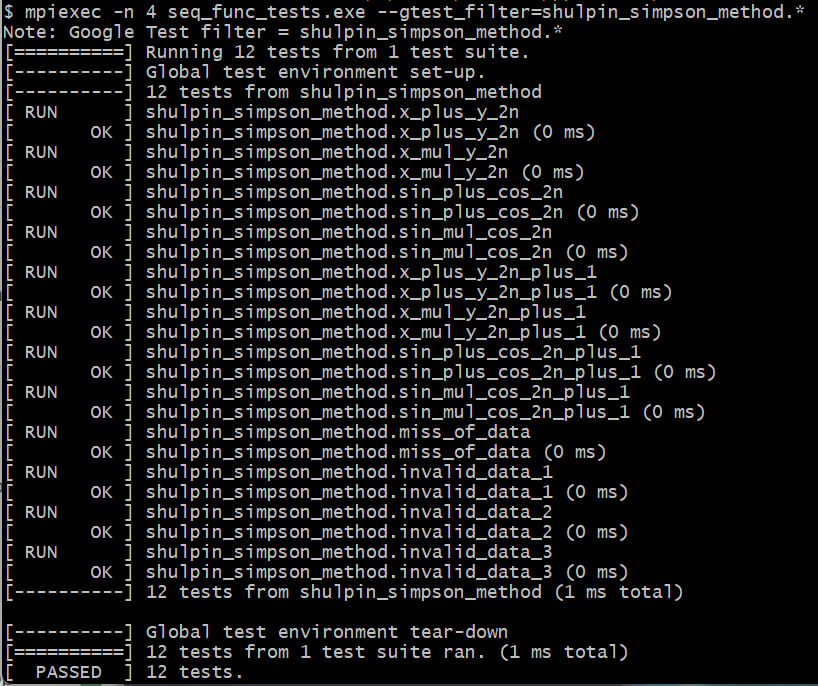
\includegraphics[height=10cm]{img/seqfunctests.jpg}
\caption{\label{fig:visualClass} Результаты тестов последовательной версии}
\end{figure}

Как видно из рисунка 1, программа успешно прошла тесты валидации, а так же тесты на проверку правильности результата. Можно приступать к проверке параллельной части.

Проводить проверку мы будем на 1, 2, 3, 4, 5, 7, 8 и 10 потоках. Все данные числа являются либо простыми, либо \(2^{n}\), либо \(10^{n}\)

\begin{figure}[H]
\centering
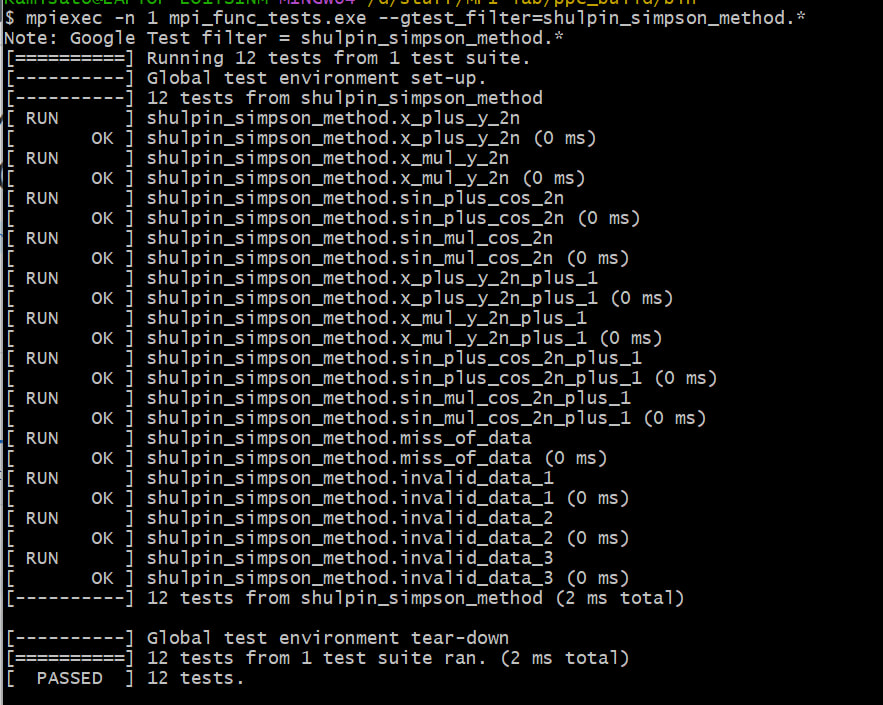
\includegraphics[height=10cm]{img/1nmpitest.jpg}
\caption{\label{fig:visualClass} Результаты тестов параллельной версии на 1 процессе}
\end{figure}

\begin{figure}[H]
\centering
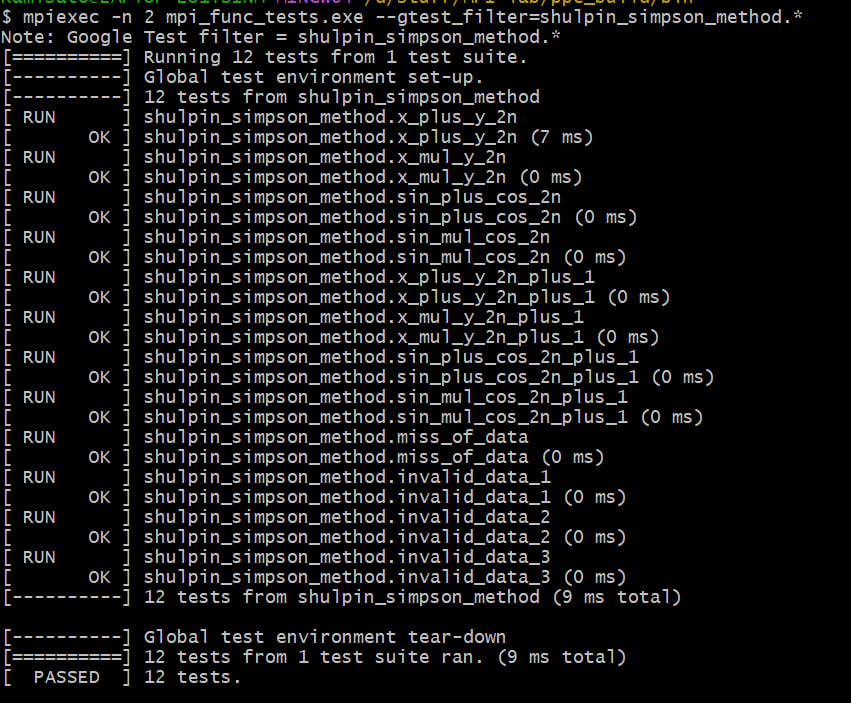
\includegraphics[height=10cm]{img/2nmpitest.jpg}
\caption{\label{fig:visualClass} Результаты тестов параллельной версии на 2 процессах}
\end{figure}

\begin{figure}[H]
\centering
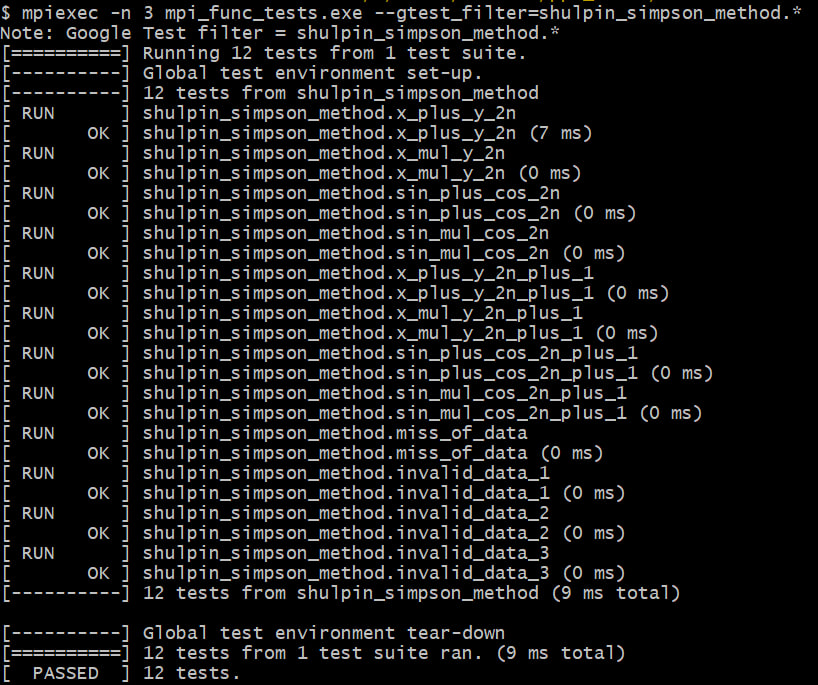
\includegraphics[height=10cm]{img/3nmpitest.jpg}
\caption{\label{fig:visualClass} Результаты тестов параллельной версии на 3 процессах}
\end{figure}

\begin{figure}[H]
\centering
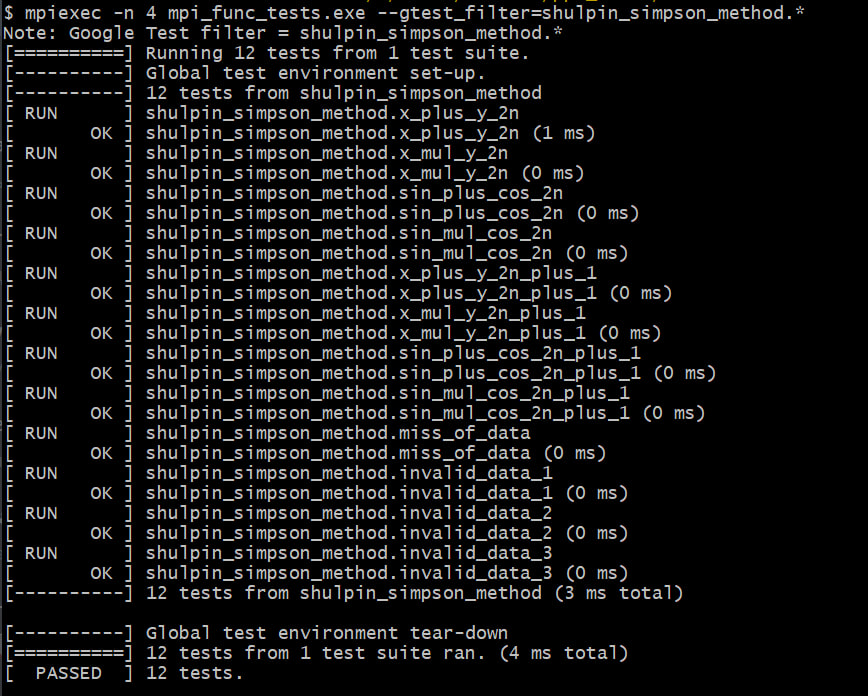
\includegraphics[height=10cm]{img/4nmpitest.jpg}
\caption{\label{fig:visualClass} Результаты тестов параллельной версии на 4 процессах}
\end{figure}

\begin{figure}[H]
\centering
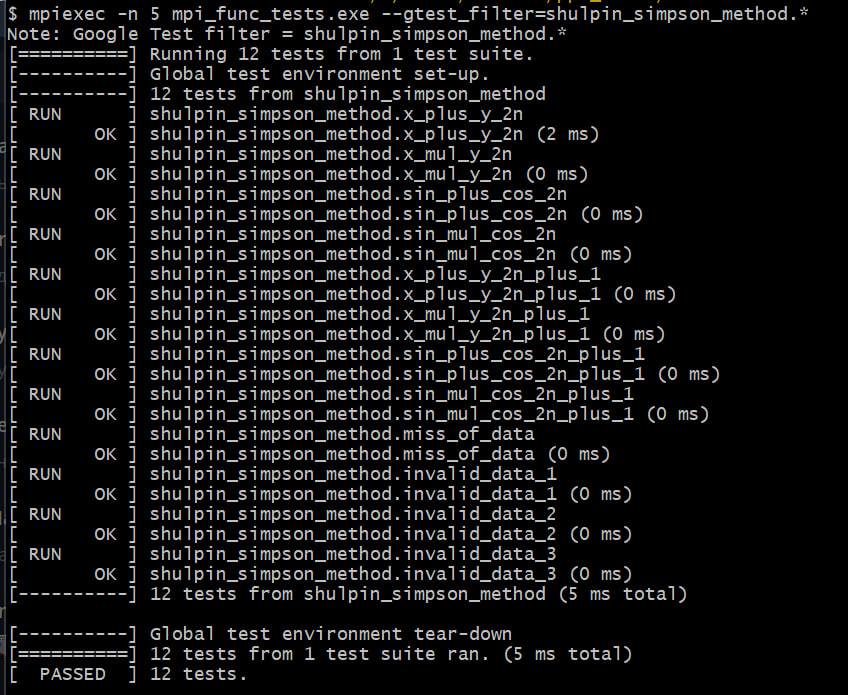
\includegraphics[height=10cm]{img/5nmpitest.jpg}
\caption{\label{fig:visualClass} Результаты тестов параллельной версии на 5 процессах}
\end{figure}

\begin{figure}[H]
\centering
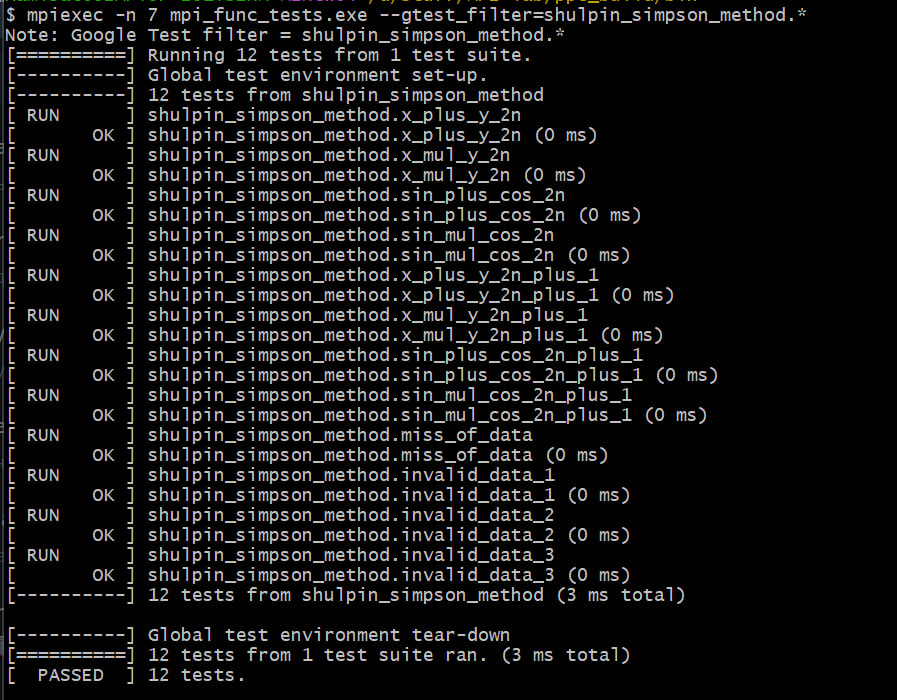
\includegraphics[height=10cm]{img/7nmpitest.jpg}
\caption{\label{fig:visualClass} Результаты тестов параллельной версии на 7 процессах}
\end{figure}

\begin{figure}[H]
\centering
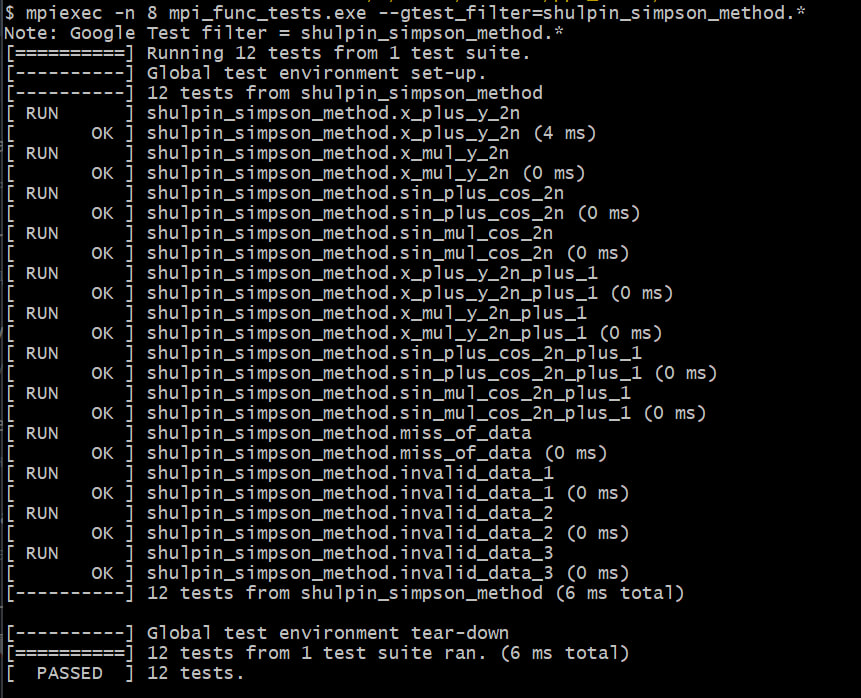
\includegraphics[height=10cm]{img/8nmpitest.jpg}
\caption{\label{fig:visualClass} Результаты тестов параллельной версии на 8 процессах}
\end{figure}

\begin{figure}[H]
\centering
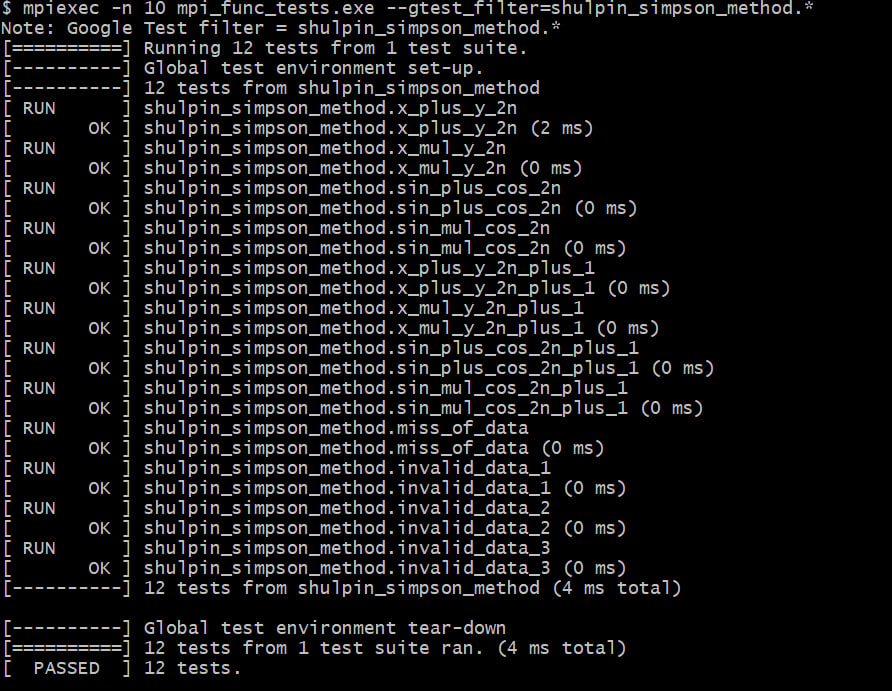
\includegraphics[height=10cm]{img/10nmpitest.jpg}
\caption{\label{fig:visualClass} Результаты тестов параллельной версии на 10 процессах}
\end{figure}

Как видно из представленных изображений, параллельная реализация успешно прошла все тесты. Теперь можно переходить к самим экспериментам

\section*{Результаты экпериментов}

В данном блоке будут представлены только результаты экспериментов. Все обсуждения будут в блоке \textbf{"Выводы из результатов"}. Тесты будем проводить на простом числе шагов интегрирования, а именно на 4201 как самом близком к \(2^n\) значении

\begin{figure}[H]
\centering
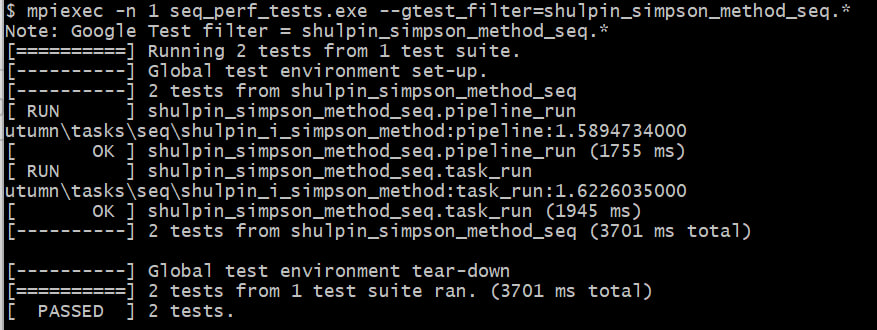
\includegraphics[height=6cm]{img/1nseqperftest.jpg}
\caption{\label{fig:visualClass} Результаты тестов производительности последовательной версии}
\end{figure}

\begin{figure}[H]
\centering
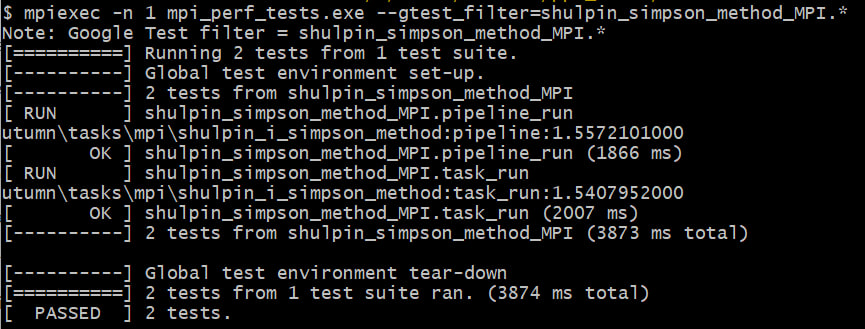
\includegraphics[height=6cm]{img/1nmpiperftest.jpg}
\caption{\label{fig:visualClass} Результаты тестов производительности параллельной версии на 1 процессе}
\end{figure}

\begin{figure}[H]
\centering
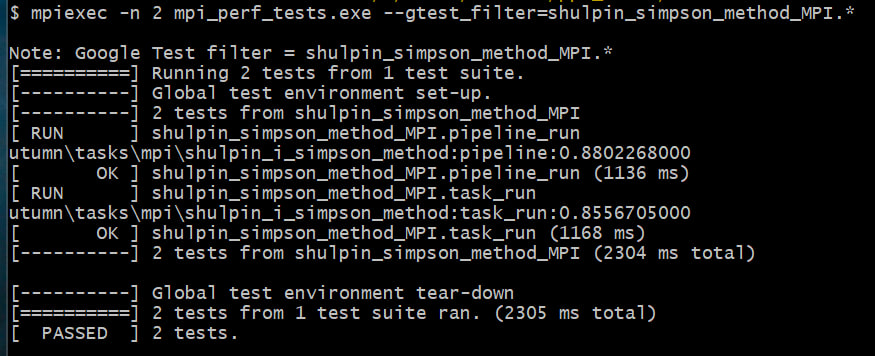
\includegraphics[height=6cm]{img/2nmpiperftest.jpg}
\caption{\label{fig:visualClass} Результаты тестов производительности параллельной версии на 2 процессах}
\end{figure}

\begin{figure}[H]
\centering
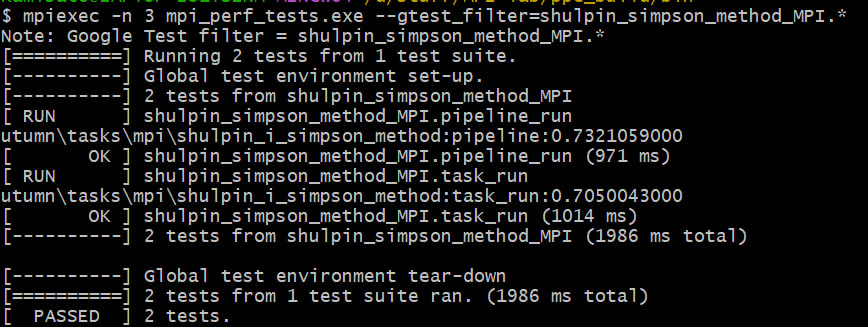
\includegraphics[height=6cm]{img/3nmpiperftest.jpg}
\caption{\label{fig:visualClass} Результаты тестов производительности параллельной версии на 3 процессах}
\end{figure}

\begin{figure}[H]
\centering
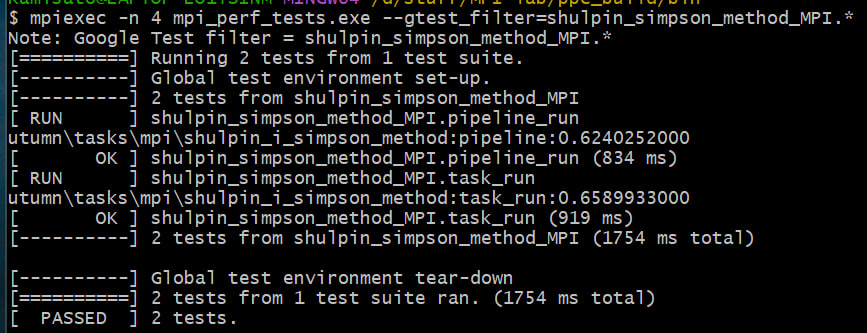
\includegraphics[height=6cm]{img/4nmpiperftest.jpg}
\caption{\label{fig:visualClass} Результаты тестов производительности параллельной версии на 4 процессах}
\end{figure}

\begin{figure}[H]
\centering
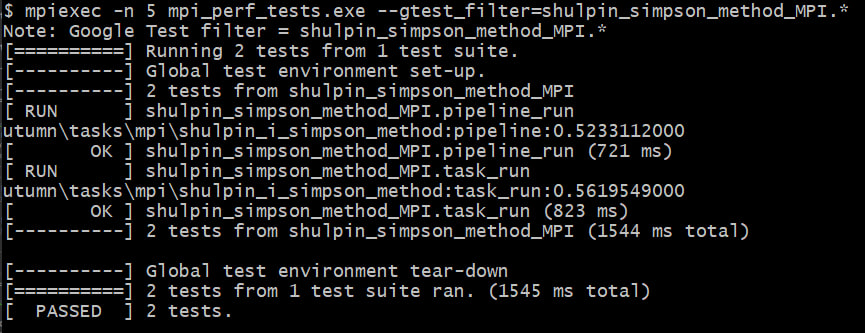
\includegraphics[height=6cm]{img/5nmpiperftest.jpg}
\caption{\label{fig:visualClass} Результаты тестов производительности параллельной версии на 5 процессах}
\end{figure}

\begin{figure}[H]
\centering
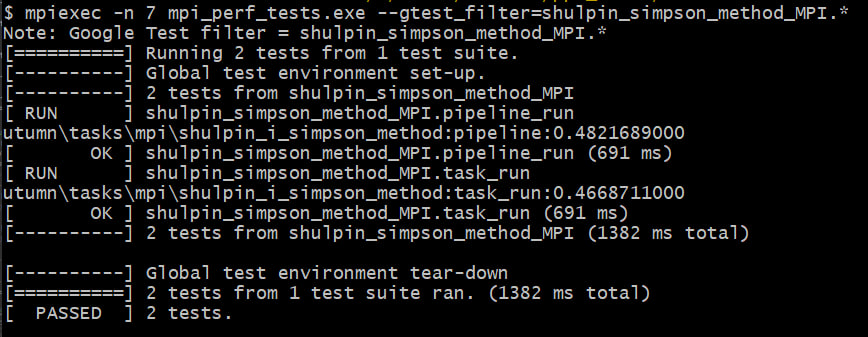
\includegraphics[height=6cm]{img/7nmpiperftest.jpg}
\caption{\label{fig:visualClass} Результаты тестов производительности параллельной версии на 7 процессах}
\end{figure}

\begin{figure}[H]
\centering
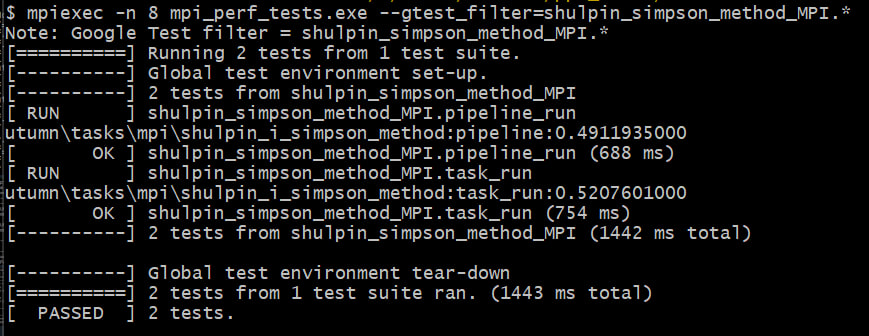
\includegraphics[height=6cm]{img/8nmpiperftest.jpg}
\caption{\label{fig:visualClass} Результаты тестов производительности параллельной версии на 8 процессах}
\end{figure}

\begin{figure}[H]
\centering
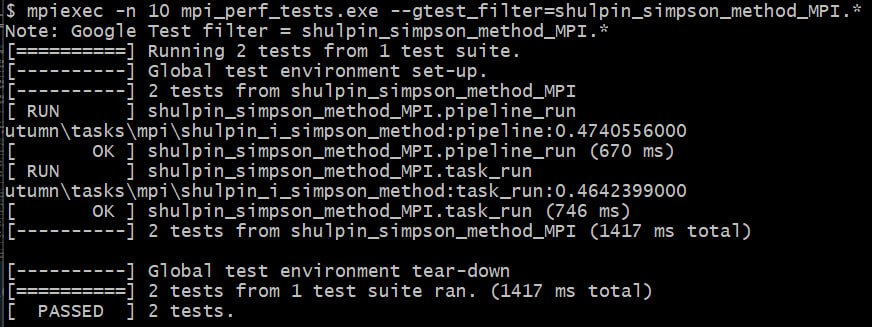
\includegraphics[height=6cm]{img/10nmpiperftest.jpg}
\caption{\label{fig:visualClass} Результаты тестов производительности параллельной версии на 10 процессах}
\end{figure}

\section*{Выводы из результатов}

Как видно из проведенных тестов, последовательная часть практически не отличается по производительности от параллельной на 1 процессе. Связяно оно с тем, что последовательная версия и параллельная с 1 процессе буквально ставновятся идентичны, ведь обрабатывают полностью все шаги метода.

Однако начиная уже с двух процессов мы видим выигрышь в работе алгоритма практически в 2 раза. В дальнейшем с ростом числа процессов время выполения будет только уменьшаться, хоть и незначительно.

Однако, на 8 процессах время выполнения неожинно выросло, относительно 7 процессов, а в дальшейшем с ростом числа процессов продолжило дальше уменьшаться. Скорее всего это связано техническими особенностями техники, на которой проводились эксперименты. Для тестов был использован Intel Core i9-13900H, в котором 6 производительных и 8 энергоэффективных ядер, и потому время выполнения увеличилось, ведь 2 энергоэффективных ядра обрабатывали код дольше.

\section*{Заключение}

В ходе данной лабораторной работы был реализован метод Симспона для вычисления значения многомерных интегралов на примере двумерного интерграла. Написаны были как последовательная и параллельная версии.

В ходе эксперимента мы убедились, что использование параллелизма значительно улучшает производительность при реализации метода Симпсона.

\newpage
\section*{Список литературы}


\begin{enumerate}
    \item Boost MPI Library Documentation: 
    \url{https://www.boost.org/doc/libs/release/libs/mpi/}
    \item Бьёрн Страуструп. «Язык программирования C++»
    \item Dr. Trefor Bazett --- Defining Double Integration with Riemann Sums | Volume under a Surface
    \url{https://www.youtube.com/watch?v=JXh9AQkKmsw}
    \item Бурден Р., Фэйрс Д. «Численные методы»
    \item Gander, W., Gautschi, W. «Adaptive Quadrature – Theory and Practice»
\end{enumerate}

\newpage
\section*{Приложение}
\begin{lstlisting}[caption={simpson\_method.hpp}]
#pragma once

#include <gtest/gtest.h>

#include <boost/mpi/collectives.hpp>
#include <boost/mpi/communicator.hpp>
#include <functional>
#include <memory>
#include <numeric>
#include <utility>

#include "core/task/include/task.hpp"

namespace shulpin_simpson_method {
using func = std::function<double(double, double)>;

double f_x_plus_y(double x, double y);
double f_x_mul_y(double x, double y);
double f_sin_plus_cos(double x, double y);
double f_sin_mul_cos(double x, double y);

double seq_simpson(double a, double b, double c, double d, int N, const func& f);
inline double calculate_coeff(const int* index, const int* limit);
double calculate_row_sum(const int* i, const int* num_steps, const double* dx, const double* dy, const double* a,
                         const double* c, const func* func);
double mpi_simpson(double a, double b, double c, double d, int N, const func& f);

class SimpsonMethodSeq : public ppc::core::Task {
 public:
  explicit SimpsonMethodSeq(std::shared_ptr<ppc::core::TaskData> taskData_) : Task(std::move(taskData_)) {};
  bool pre_processing() override;
  bool validation() override;
  bool run() override;
  bool post_processing() override;
  void set_seq(const func& f);

 private:
  double a_seq;
  double b_seq;
  double c_seq;
  double d_seq;
  int N_seq;
  func func_seq;
  double res_seq;
};

class SimpsonMethodMPI : public ppc::core::Task {
 public:
  explicit SimpsonMethodMPI(std::shared_ptr<ppc::core::TaskData> taskData_) : Task(std::move(taskData_)) {};
  bool pre_processing() override;
  bool validation() override;
  bool run() override;
  bool post_processing() override;
  void set_MPI(const func& f);

 private:
  double a_MPI;
  double b_MPI;
  double c_MPI;
  double d_MPI;
  int N_MPI;
  func func_MPI;
  double res_MPI;
  boost::mpi::communicator world;
};
}  // namespace shulpin_simpson_method
\end{lstlisting}

\begin{lstlisting}[caption={simpson\_method.cpp}]
#include "mpi/shulpin_i_simpson_method/include/simpson_method.hpp"

#include <algorithm>
#include <boost/mpi.hpp>
#include <boost/mpi/collectives.hpp>
#include <cmath>
#include <functional>

double shulpin_simpson_method::f_x_plus_y(double x, double y) { return x + y; }
double shulpin_simpson_method::f_x_mul_y(double x, double y) { return x * y; }
double shulpin_simpson_method::f_sin_plus_cos(double x, double y) { return std::sin(x) + std::cos(y); }
double shulpin_simpson_method::f_sin_mul_cos(double x, double y) { return std::sin(x) * std::cos(y); }

inline double shulpin_simpson_method::calculate_coeff(const int* index, const int* limit) {
  if (*index == 0 || *index == *limit) {
    return 1.0;
  }
  return (*index % 2 == 0) ? 2.0 : 4.0;
}

double shulpin_simpson_method::calculate_row_sum(const int* i, const int* num_steps, const double* dx, const double* dy,
                                                 const double* a, const double* c, const func* func) {
  double row_sum = 0.0;
  double x = *a + (*i) * (*dx);
  double x_coeff = calculate_coeff(i, num_steps);

  for (int j = 0; j <= *num_steps; ++j) {
    double y = *c + j * (*dy);
    row_sum += x_coeff * calculate_coeff(&j, num_steps) * (*func)(x, y);
  }

  return row_sum;
}

double shulpin_simpson_method::seq_simpson(double a, double b, double c, double d, int N, const func& func_seq) {
  if (N % 2 != 0) {
    ++N;
  }

  double dx = (b - a) / N;
  double dy = (d - c) / N;
  double seq_sum = 0.0;

  for (int i = 0; i <= N; ++i) {
    seq_sum += calculate_row_sum(&i, &N, &dx, &dy, &a, &c, &func_seq);
  }

  return (dx * dy / 9.0) * seq_sum;
}

double shulpin_simpson_method::mpi_simpson(double a, double b, double c, double d, int N, const func& func_MPI) {
  boost::mpi::communicator world;
  int num_procs = world.size();
  int rank = world.rank();

  int num_steps = N;
  if (num_steps % 2 != 0) {
    ++num_steps;
  }

  double dx = (b - a) / num_steps;
  double dy = (d - c) / num_steps;

  int chunk_size = num_steps / num_procs;
  int extra_rows = num_steps % num_procs;

  int local_start = rank * chunk_size + std::min(rank, extra_rows);
  int local_end = local_start + chunk_size - 1;

  if (rank < extra_rows) {
    ++local_end;
  } else if (rank == num_procs - 1) {
    local_end = num_steps;
  }

  double local_sum = 0.0;

  for (int i = local_start; i <= local_end; ++i) {
    local_sum += calculate_row_sum(&i, &num_steps, &dx, &dy, &a, &c, &func_MPI);
  }

  double global_sum = 0.0;
  if (rank == 0) {
    global_sum = local_sum;
    for (int i = 1; i < num_procs; ++i) {
      double recv_sum;
      world.recv(i, 0, recv_sum);
      global_sum += recv_sum;
    }
    return (dx * dy / 9.0) * global_sum;
  }

  world.send(0, 0, local_sum);
  return 0.0;
}

bool shulpin_simpson_method::SimpsonMethodSeq::pre_processing() {
  internal_order_test();

  double a_value = *reinterpret_cast<double*>(taskData->inputs[0]);
  double b_value = *reinterpret_cast<double*>(taskData->inputs[1]);
  double c_value = *reinterpret_cast<double*>(taskData->inputs[2]);
  double d_value = *reinterpret_cast<double*>(taskData->inputs[3]);
  int N_value = *reinterpret_cast<int*>(taskData->inputs[4]);

  a_seq = a_value;
  b_seq = b_value;
  c_seq = c_value;
  d_seq = d_value;
  N_seq = N_value;

  return true;
}

bool shulpin_simpson_method::SimpsonMethodSeq::validation() {
  internal_order_test();

  return ((taskData->inputs.size() == 5) && (*reinterpret_cast<int*>(taskData->inputs[4]) > 0) &&
          (*reinterpret_cast<double*>(taskData->inputs[0]) < *reinterpret_cast<double*>(taskData->inputs[1])) &&
          (*reinterpret_cast<double*>(taskData->inputs[2]) < *reinterpret_cast<double*>(taskData->inputs[3])));
}

bool shulpin_simpson_method::SimpsonMethodSeq::run() {
  internal_order_test();

  res_seq = seq_simpson(a_seq, b_seq, c_seq, d_seq, N_seq, func_seq);

  return true;
}

bool shulpin_simpson_method::SimpsonMethodSeq::post_processing() {
  internal_order_test();
  reinterpret_cast<double*>(taskData->outputs[0])[0] = res_seq;

  return true;
}

bool shulpin_simpson_method::SimpsonMethodMPI::pre_processing() {
  internal_order_test();
  if (world.rank() == 0) {
    double a_value = *reinterpret_cast<double*>(taskData->inputs[0]);
    double b_value = *reinterpret_cast<double*>(taskData->inputs[1]);
    double c_value = *reinterpret_cast<double*>(taskData->inputs[2]);
    double d_value = *reinterpret_cast<double*>(taskData->inputs[3]);
    int N_value = *reinterpret_cast<int*>(taskData->inputs[4]);

    a_MPI = a_value;
    b_MPI = b_value;
    c_MPI = c_value;
    d_MPI = d_value;
    N_MPI = N_value;
  }

  return true;
}

bool shulpin_simpson_method::SimpsonMethodMPI::validation() {
  internal_order_test();

  if (world.rank() == 0) {
    return ((taskData->inputs.size() == 5) && (*reinterpret_cast<int*>(taskData->inputs[4]) > 0) &&
            (*reinterpret_cast<double*>(taskData->inputs[0]) < *reinterpret_cast<double*>(taskData->inputs[1])) &&
            (*reinterpret_cast<double*>(taskData->inputs[2]) < *reinterpret_cast<double*>(taskData->inputs[3])));
  }

  return true;
}

bool shulpin_simpson_method::SimpsonMethodMPI::run() {
  internal_order_test();

  double local_res{};

  boost::mpi::broadcast(world, a_MPI, 0);
  boost::mpi::broadcast(world, b_MPI, 0);
  boost::mpi::broadcast(world, c_MPI, 0);
  boost::mpi::broadcast(world, d_MPI, 0);
  boost::mpi::broadcast(world, N_MPI, 0);

  local_res = mpi_simpson(a_MPI, b_MPI, c_MPI, d_MPI, N_MPI, func_MPI);

  boost::mpi::reduce(world, local_res, res_MPI, std::plus<>(), 0);
  return true;
}

bool shulpin_simpson_method::SimpsonMethodMPI::post_processing() {
  internal_order_test();
  if (world.rank() == 0) {
    reinterpret_cast<double*>(taskData->outputs[0])[0] = res_MPI;
  }

  return true;
}

void shulpin_simpson_method::SimpsonMethodSeq::set_seq(const func& f) { func_seq = f; }

void shulpin_simpson_method::SimpsonMethodMPI::set_MPI(const func& f) { func_MPI = f; }
\end{lstlisting}

\end{document}
